\documentclass[12pt]{beamer}
\usepackage{../Estilos/BeamerMAF}
\usepackage{../Estilos/ColoresLatex}
%Sección para el tema de beamer, con el theme, usercolortheme y sección de footers
\usetheme{Frankfurt}
\usecolortheme{beaver}
%\useoutertheme{default}
\setbeamercovered{invisible}
% or whatever (possibly just delete it)
\setbeamertemplate{section in toc}[sections numbered]
\setbeamertemplate{subsection in toc}[subsections numbered]
\setbeamertemplate{subsection in toc}{\leavevmode\leftskip=3.2em\rlap{\hskip-2em\inserttocsectionnumber.\inserttocsubsectionnumber}\inserttocsubsection\par}
% \setbeamercolor{section in toc}{fg=blue}
% \setbeamercolor{subsection in toc}{fg=blue}
% \setbeamercolor{frametitle}{fg=blue}
\setbeamertemplate{caption}[numbered]

\setbeamertemplate{footline}
\beamertemplatenavigationsymbolsempty
\setbeamertemplate{headline}{}


\makeatletter
% \setbeamercolor{section in foot}{bg=gray!30, fg=black!90!orange}
% \setbeamercolor{subsection in foot}{bg=blue!30!yellow, fg=red}
% \setbeamercolor{date in foot}{bg=black, fg=white}
\setbeamertemplate{footline}
{
  \leavevmode%
  \hbox{%
  \begin{beamercolorbox}[wd=.333333\paperwidth,ht=2.25ex,dp=1ex,center]{section in foot}%
    \usebeamerfont{section in foot} \insertsection
  \end{beamercolorbox}%
  \begin{beamercolorbox}[wd=.333333\paperwidth,ht=2.25ex,dp=1ex,center]{subsection in foot}%
    \usebeamerfont{subsection in foot}  \insertsubsection
  \end{beamercolorbox}%
  \begin{beamercolorbox}[wd=.333333\paperwidth,ht=2.25ex,dp=1ex,right]{date in head/foot}%
    \usebeamerfont{date in head/foot} \insertshortdate{} \hspace*{2em}
    \insertframenumber{} / \inserttotalframenumber \hspace*{2ex} 
  \end{beamercolorbox}}%
  \vskip0pt%
}







\setbeamercolor{section in foot}{bg=forestgreen(web), fg=white}
\setbeamercolor{subsection in foot}{bg=frenchlilac, fg=white}
\setbeamercolor{date in foot}{bg=blue, fg=white}

\makeatletter
\setbeamertemplate{footline}
{
\leavevmode%
\hbox{%
\begin{beamercolorbox}[wd=.333333\paperwidth,ht=2.25ex,dp=1ex,center]{section in foot}%
  \usebeamerfont{section in foot} \insertsection
\end{beamercolorbox}%
\begin{beamercolorbox}[wd=.333333\paperwidth,ht=2.25ex,dp=1ex,center]{subsection in foot}%
  \usebeamerfont{subsection in foot}  \insertsubsection
\end{beamercolorbox}%
\begin{beamercolorbox}[wd=.333333\paperwidth,ht=2.25ex,dp=1ex,right]{date in head/foot}%
  \usebeamerfont{date in head/foot} \insertshortdate{} \hspace*{1.5em}
  \insertframenumber{} / \inserttotalframenumber \hspace*{2ex} 
\end{beamercolorbox}}%
\vskip0pt%
}
\makeatother
\usefonttheme{serif}
\setbeamercolor{frametitle}{bg=palerobineggblue}
\resetcounteronoverlays{saveenumi}

\date{29 de abril de 2022}

\title{\large{Esferas y la ecuación de Legendre}}
\subtitle{Funciones Especiales I}
\author{M. en C. Gustavo Contreras Mayén}

\begin{document}
\maketitle
\fontsize{14}{14}\selectfont
\spanishdecimal{.}

\section*{Contenido}
\frame[allowframebreaks]{\tableofcontents[currentsection, hideallsubsections]}

\section{Ecuación de Laplace}
\frame{\tableofcontents[currentsection, hideothersubsections]}
\subsection{Coordenadas esféricas}

\begin{frame}
\frametitle{Laplace en simetría esférica}
Para resolver la ecuación de Laplace:
\pause
\begin{align*}
\laplacian{\Psi} = 0
\end{align*}
en un sistema coordenado esférico $(r, \theta, \varphi)$, hacemos el cambio entre el sistema cartesiano y el esférico.
\end{frame}
\begin{frame}
\frametitle{Expresión en coord. esféricas}
Teniendo entonces:
\pause
\begin{align}
\begin{aligned}[b]
\dfrac{1}{r^{2}} \pdv{r} \left( r^{2} \pdv{\Psi}{r} \right) &+ \dfrac{1}{r^{2} \, \sin \theta} \bigg[ \pdv{\theta} \left( \sin \theta \pdv{\Psi}{\theta} \right) + \\[0.5em]
&+ \dfrac{1}{\sin \theta} \, \pdv[2]{\Psi}{\varphi} \bigg] = 0
\end{aligned}
\label{eq:ecuacion_22_15}
\end{align}
\end{frame}

\subsection{Separación de variables}

\begin{frame}
\frametitle{Solución propuesta}
Para ocupar la técnica de separación de variables, proponemos una solución del tipo:
\pause
\begin{align*}
\Psi(r, \theta, \varphi) = R(r) \, \Theta \, (\theta) \, \Phi(\varphi)
\end{align*}
Que sustituimos en la ec (\ref{eq:ecuacion_22_15}), y cuyo procedimiento ya sabemos realizar.
\end{frame}
\begin{frame}
\frametitle{Ec. Laplace en coord. esféricas}
Tenemos que:
\pause
\begin{align*}
\Theta \Phi \dfrac{1}{r^{2}} \, \dv{r} \left( r^{2} \dv{R}{r} \right) &+ \dfrac{R}{r^{2}} \bigg[ \dfrac{\Phi}{\sin \theta} \, \dv{\theta} \left( \sin \theta \dv{\Theta}{\theta} \right) + \\[0.5em]
&+ \dfrac{\Theta}{\sin^{2} \theta} \, \dv[2]{\Phi}{\varphi} \bigg] = 0
\end{align*}
donde cada derivada se realiza sobre cada una de las variables.
\end{frame}
\begin{frame}
\frametitle{Simplificando la expresión}
Al dividir entre $R \, \Theta \, \Phi$ y luego multiplicar por $r^{2}$, llegamos a:
\pause
\begin{align*}
\dfrac{1}{R} \, \dv{r} \left( r^{2} \dv{R}{r} \right) &+ \bigg[ \dfrac{1}{\Theta \sin \theta} \, \dv{\theta} \left( \sin \theta \dv{\Theta}{\theta} \right) + \\[0.5em]
&+ \dfrac{1}{\Phi \sin^{2} \theta} \, \dv[2]{\Phi}{\varphi} \bigg] = 0
\end{align*}
\end{frame}
\begin{frame}
\frametitle{Constante de separación}
Ya que cada uno de los términos es función de variables independientes, por tanto deben de ser una constante, y las dos constantes deben de sumar cero.
\\
\bigskip
\pause
Así obtenemos:
\pause
\begin{align*}
\dfrac{1}{R} \, \dv{r} \left( r^{2} \dv{R}{r} \right) &= \alpha \\[0.5em]
\dfrac{1}{\Theta \sin \theta} \, \dv{\theta} \left( \sin \theta \dv{\Theta}{\theta} \right) + \dfrac{1}{\Phi \sin^{2} \theta} \, \dv[2]{\Phi}{\varphi} &= - \alpha
\end{align*}
\end{frame}
\begin{frame}
\frametitle{Nueva separación en una ecuación}
La segunda ecuación debe de separarse nuevamente, agregamos $\alpha$ en ambos lados de la expresión y multiplicamos por $\sin^{2} \theta$, llegando a:
\pause
\begin{align*}
\dfrac{\sin \theta}{\Theta} \, \dv{\theta} &\left( \sin \theta \dv{\Theta}{\theta} \right) + \\[0.5em]
&+\alpha \, \sin^{2} \theta +  \dfrac{1}{\Phi} \, \dv[2]{\Psi}{\varphi} = 0
\end{align*}
\end{frame}
\begin{frame}
\frametitle{Segunda constante de separación}
Siguiendo el mismo razonamiento, tendremos una segunda constante de separación:
\pause
\begin{align*}
\dfrac{\sin \theta}{\Theta} \, \dv{\theta} \left( \sin \theta \dv{\Theta}{\theta} \right) &= \beta \\[0.5em]
\dfrac{1}{\Phi} \, \dv[2]{\Phi}{\varphi} = - \beta
\end{align*}
\end{frame}
\begin{frame}
\frametitle{Sistema de EDO2H}
De modo que hemos recuperado tres EDO2H, cada una de una sola variable:
\pause
\begin{eqnarray}
\dfrac{1}{r^{2}} \, \dv{r} \left( r^{2} \dv{R}{r} \right) - \dfrac{\alpha}{r^{2}} \, R &=& 0 \label{eq:ecuacion_22_17a} \\[0.5em] \pause
\dfrac{1}{\sin \theta} \, \dv{\theta} \left( \sin \theta \dv{\Theta}{\theta} \right) + \left( \alpha - \dfrac{\beta}{\sin^{2} \theta} \right) \, \Theta &=& 0 \label{eq:ecuacion_22_17b} \\[0.5em] \pause
\dv[2]{\Phi}{\varphi} + \beta \, \Phi &=& 0 \label{eq:ecuacion_22_17c}
\end{eqnarray}
\end{frame}
\begin{frame}
\frametitle{Identificando las EDO2H}
\setbeamercolor{item projected}{bg=ballblue,fg=white}
\setbeamertemplate{enumerate items}{%
\usebeamercolor[bg]{item projected}%
\raisebox{1.5pt}{\colorbox{bg}{\color{fg}\footnotesize\insertenumlabel}}%
}
\begin{enumerate}[<+->]
\item La ec. (\ref{eq:ecuacion_22_17a}) se conoce como \textbf{ecuación radial}.
\item La ec. (\ref{eq:ecuacion_22_17b}) es la \textbf{ecuación polar}.
\item La tercera ec. (\ref{eq:ecuacion_22_17c}) es la \textbf{ecuación azimutal}.
\end{enumerate}
\end{frame}

\subsection{Simetría azimutal}

\begin{frame}
\frametitle{Caso de simetría angular}
Consideramos el caso donde $\Phi$ es la función constante, \pause esto corresponde a problemas con una \emph{simetría azimutal}, \pause es decir, problemas para los cuales está claro \emph{a priori} que el potencial es independiente del ángulo azimutal $\varphi$.
\end{frame}
\begin{frame}
\frametitle{Coordenada constante}
En tales situaciones, la ec. \ref{eq:ecuacion_22_17c}) implica que $\beta = 0$ porque $\Phi$ es una constante (distinta de cero).
\\
\bigskip
\pause
Las variables independientes se reducen a dos: 
\begin{align*}
\psi (r, \theta) = R (r) \, \Theta (\theta)    
\end{align*}
\end{frame}
\begin{frame}
\frametitle{Sistema de EDO2H}
Se reduce a un sistema de dos EDO2H:
\pause
\begin{eqnarray}
\begin{aligned}
\dfrac{1}{r^{2}} \dv{r} \left( r^{2} \dv{R}{r} \right) - \dfrac{\alpha}{r^{2}} \, R &= 0 \\[0.5em]  \pause
\dfrac{1}{\sin \theta} \dv{\theta} \left( \sin \theta \dv{\Theta}{\theta} \right) + \alpha \, \Theta &= 0
\end{aligned}
\label{eq:ecuacion_26_02}
\end{eqnarray}
\end{frame}

\subsection{Resolviendo las EDO2H.}

\begin{frame}
\frametitle{Ecuación polar}
De manera inicial nos enfocamos en la ecuación polar.
\\
\bigskip
\pause
La presencia en el denominador del término $\sin \theta \dd{\theta}$ (que es el diferencial de $\cos \theta)$ sugiere el cambio de variable de $\theta$ a $u \equiv \cos \theta$.
\end{frame}
\begin{frame}
\frametitle{Diferenciando la función}
Para cualquier función $f (\theta)$, con la regla de la cadena se tiene:
\pause
\begin{eqnarray*}
\begin{aligned}
\dv{f}{u} &= \dv{f}{\theta} \dv{\theta}{u} = \\[0.5em] \pause
&= \dv{f}{\theta} \dfrac{1}{\dv*{u}{\theta}} = \\[0.5em] \pause
&= - \dfrac{1}{\sin \theta} \dv{f}{\theta}
\end{aligned}
\end{eqnarray*}
\end{frame}
\begin{frame}
\frametitle{Expresión equivalente}
De manera equivalente:
\pause
\begin{align}
\dv{f}{\theta} = - \sin \theta \dv{f}{u}
\label{eq:ecuacion_26_03}
\end{align}
\pause
Esto nos permite convertir la derivada de una función con respecto a $u$, en la derivada de la misma función con respecto a $\theta$.
\end{frame}
\begin{frame}
\frametitle{Proponiendo una función}
Proponemos una función $P(u)$ tal que:
\pause
\begin{align*}
P(u) = \Theta(\theta)
\end{align*}
Usamos la regla de la cadena mostrada, sustituyendo en la ecuación polar y escribiendo $\sin^{2} \theta = 1 - u^{2}$.
\end{frame}
\begin{frame}
\frametitle{Ecuación diferencial obtenida}
La EDO pasa a ser:
\pause
\begin{align*}
- \dfrac{1}{\sin \theta} \dv{\theta} \bigg[ (1 - u^{2}) \dv{P}{u} \bigg] + \alpha \, P = 0
\end{align*}
El término en el corchete es función de $u$.
\end{frame}
\begin{frame}
\frametitle{Cambiando la derivada}
Ocupando la ec. (\ref{eq:ecuacion_26_03}), podemos convertir la derivada en $\theta$ en una derivada en $u$, para así obtener:
\pause
\begin{align}
\dv{u} \bigg[ (1 - u^{2}) \dv{P}{u} \bigg] + \alpha P = 0
\label{eq:ecuacion_26_04}
\end{align}
\end{frame}
\begin{frame}
\frametitle{Ecuación diferencial}
Que se puede escribir como:
\pause
\begin{align}
(1 - u^{2}) \, \dv[2]{P}{u} - 2 \, u \, \dv{P}{u} + \alpha \, P = 0
\label{eq:ecuacion_26_05}
\end{align}
\end{frame}
\begin{frame}
\frametitle{Misma ED escrita de otra manera}
De manera equivalente:
\pause
\begin{align}
\dv[2]{P}{u} - \dfrac{2 \, u}{1 - u^{2}} \, \dv{P}{u} + \dfrac{\alpha}{(1 - u^{2})} \, P = 0
\label{eq:ecuacion_26_06}
\end{align}
A esta ecuación (\ref{eq:ecuacion_26_05}) - (\ref{eq:ecuacion_26_06}) se le conoce como la \textbf{\textcolor{lava}{ecuación diferencial de Legendre}}.
\end{frame}
\begin{frame}
\frametitle{Solución a la ED de Legendre}
Las soluciones a la ecuación de Legendre son los polinomios de Legendre de orden $n$: $P_{n} (x)$, y se detallan en las notas de trabajo, por lo que aquí haremos uso de las mismas y de sus propiedades.
\end{frame}

\subsection{Ecuación radial}

\begin{frame}
\frametitle{Eligiendo la constante de separación}
En la solución de la ecuación angular, se determina que $\alpha = k (k + 1)$, de esta manera la ecuación radial se escribe como:
\pause
\begin{align}
r^{2} \dv[2]{R}{r} + 2 R \dv{R}{r} - k(k + 1) R = 0
\label{eq:ecuacion_26_28}
\end{align}
\end{frame}
\begin{frame}
\frametitle{Solución propuesta}
Como $p_{2} (0) = 0$, se considera una solución a la ecuación radial de la forma:
\pause
\begin{align*}
R(r) = r^{s} \nsum_{n=0}^{\infty} b_{n} \, r^{n}
\end{align*}
\pause
es decir, hacemos un desarrollo con el método de Frobenius.
\end{frame}
\begin{frame}
\frametitle{Solución con el método de Frobenius}
La solución general a la ecuación radial es entonces:
\pause
\begin{align*}
R_{k}(r) \equiv A_{k} \, r^{k} + \dfrac{B_{k}}{r^{k+1}} \hspace{0.3cm} k = 0, 1, 2, \ldots
\end{align*}
con $A_{k}$ y $B_{k}$ coeficientes por determinar.
\end{frame}

\subsection{Solución completa}

\begin{frame}
\frametitle{La solución completa a la EDO}
Para encontrar la solución general a la ecuación de Laplace en coordenadas esféricas con una simetría azimutal, multiplicamos la solución radial y angular (dada por los polinomios de Legendre) para cada $k$ y se suma en todos los valores posibles de $k$:
\pause
\begin{align}
\psi(r, \theta) = \nsum_{k=0}^{\infty} \left( A_{k} \, r^{k} + \dfrac{B_{k}}{r^{k+1}} \right) \, P_{k} (\cos \theta)
\label{eq:ecuacion_26_29}
\end{align}
donde se ha cambiado $\cos \theta$ por $u$.
\end{frame}


\section{Esferas y temperaturas}
\frame{\tableofcontents[currentsection, hideothersubsections]}
\subsection{Planteamiento}

\begin{frame}
\frametitle{Enunciado}
Dos hemisferios sólidos conductores de calor de radio $a$, separados por un pequeño espacio aislante, forman una esfera.
\\
\bigskip
\pause
Las dos mitades de la esfera están en contacto en el exterior, con dos baños de calor (infinitos) a temperaturas $T_{0}$ y $-T_{0}$.
\end{frame}
\begin{frame}
\frametitle{Figura de los hemisferios de la esfera}
\begin{figure}[H]
    \centering
    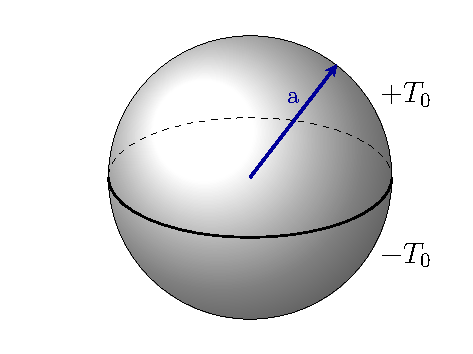
\includegraphics[scale=1.2]{Imagenes/Ejemplo_Esfera_01.eps}
    % \caption{Dos hemisferios a distintas temperaturas.}
    % \label{fig:figura_esfera_01}
\end{figure}
\end{frame}
\begin{frame}
\frametitle{Problema a resolver}
\textbf{Queremos encontrar la distribución de temperatura $T (r, \theta, \varphi)$ en puntos dentro de la esfera.}
\end{frame}
\begin{frame}
\frametitle{Uso de la expresión obtenida}
Ya tenemos una expresión que nos permitirá resolver el ejercicio, considerando algunos puntos importantes.
\\
\bigskip
\pause
En este ejercicio se muestra que es muy importante tomar en cuenta las características que presenta un problema: geometría involucrada, ecuación que modela el fenómeno, técnica de solución a la ecuación, etc.
\end{frame}

\subsection*{Identificando puntos importantes.}

\begin{frame}
\frametitle{Ajustando el problema a la geometría}
Elegimos un sistema de coordenadas esféricas en el que el origen coincide con el centro de la esfera y el eje polar es perpendicular al plano ecuatorial.
\\
\bigskip
\pause
Suponemos que el hemisferio con temperatura $T_{0}$ es el hemisferio norte, el hemisferio sur está a la temperatura $-T_{0}$.
\end{frame}
\begin{frame}
\frametitle{Ventaja de la simetría}
Dado que el problema tiene simetría azimutal, \pause $T$ es independiente de $\varphi$, y podemos escribir inmediatamente la solución general con simetría azimutal de la ecuación Laplace en coordenadas esféricas:
\pause
\begin{align*}
\psi (r, \theta) = \nsum_{k=0}^{\infty} \left( A_{k} \, r^{k} + \dfrac{B_{k}}{r^{k+1}} \right) \, P_{k} (\cos \theta)
\end{align*}
\end{frame}
\begin{frame}
\frametitle{Estudiando el punto $r = 0$}
Sin embargo, dado que el origen $r = 0$ está en la región de interés, \pause debemos excluir todos los potencias negativas de $r$.
\\
\bigskip
\pause
Esto se logra haciendo que $B_{k} = 0$.
\end{frame}
\begin{frame}
\frametitle{Expresión para el problema}
Así, tenemos que:
\pause
\begin{align}
T (r, \theta) = \nsum_{n=0}^{\infty} A_{n} \, r^{n} \, P_{n} (\cos \theta)
\label{eq:ecuacion_26_50}
\end{align}
\pause
Quedando pendiente el cálculo de los coeficientes $A_{n}$.
\end{frame}
\begin{frame}
\frametitle{Calculando los coeficientes}
Para resolver esta parte, revisemos que:
\pause
\begin{align*}
T (a, \theta) = \begin{cases}
T_{0} & \mbox{ si } 0 \leq \theta < \dfrac{\pi}{2} \\[1em]
-T_{0} & \mbox{ si } \dfrac{\pi}{2} < \theta \leq \pi
\end{cases}
\end{align*}
\end{frame}
\begin{frame}
\frametitle{Cambiando la variable}
En términos de $u = \cos \theta$, queda expresado por:
\pause
\begin{align}
\begin{aligned}
T (a, u) &= \begin{cases}
-T_{0} & \mbox{ si } -1 \leq u < 0 \\[1em]
T_{0} & \mbox{ si } 0 < u \leq 1
\end{cases} = \\[0.5em]
&= \nsum_{n=0}^{\infty} A_{n} \, a_{n} \, P_{n} (u)
\end{aligned}
\label{eq:ecuacion_26_51}
\end{align}
\end{frame}
\begin{frame}
\frametitle{Usando las notas de trabajo}
Excepto por el uso de $u$ en lugar de $x$, \pause es completamente equivalente a la expansión del ejemplo que se encuentra en las notas de trabajo.
\\
\bigskip
\pause
Encontramos que los coeficientes pares están ausentes y:
\begin{align*}
c_{2k+1} \equiv A_{2k+1} \, a^{2k+1} = \dfrac{(-1)^{k} (4 \, k + 3)(2 \, k)!}{2^{2k+1} \, k! \, (k+1)!} \, T_{0}
\end{align*}
\end{frame}
\begin{frame}
\frametitle{Despejando los coeficientes}
Despejando $A_{2k+1}$ de la ecuación anterior, para utilizarlo dentro de la ec. (\ref{eq:ecuacion_26_50}) \pause nos lleva a la solución, que \emph{determina la temperatura en puntos interiores de la esfera}:
\end{frame}
\begin{frame}
\frametitle{Solución al ejercicio}
\begin{align}
\begin{aligned}
T (r, \theta) = T_{0} \, \nsum_{k=0}^{\infty} &\dfrac{(-1)^{k} (4 \, k {+} 3)(2 \, k)!}{2^{2k+1} \, k! \, (k {+} 1)!} \times \\[0.5em]
&\times \left( \dfrac{r}{a} \right)^{2k+1} \, P_{2k+1} (\cos \theta)
\end{aligned}
\label{eq:ecuacion_26_52}
\end{align}
donde se ha sustituido $\cos \theta$ por $u$.
\end{frame}

\section{Esferas y potenciales}
\frame{\tableofcontents[currentsection, hideothersubsections]}
\subsection{Entendiendo el ejercicio}

\begin{frame}
\frametitle{Planteamiento del ejercicio}
Considere dos hemisferios eléctricamente conductores de radio $a$ separados por un pequeño espacio aislante en el ecuador. 
\\
\bigskip
\pause
El hemisferio superior se mantiene en el potencial $V_{0}$ y el inferior en $-V_{0}$.
\end{frame}
\begin{frame}
\frametitle{Descripción gráfica del problema}
\begin{figure}[H]
    \centering
    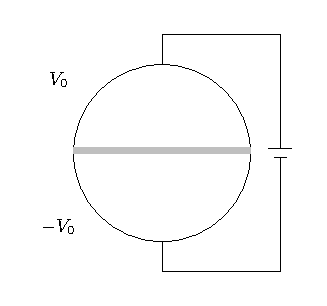
\includegraphics[scale=1]{Imagenes/Ejemplo_Esfera_03.eps}
    \caption{Dos hemisferios conductores cada uno con un potencial. El hemisferio superior tiene un rango para el ángulo polar $0 \leq \theta < \pi/2$ o $0 < \cos \theta \leq 1$, mientras que el hemisferio inferior tiene el rango $\pi/2 < \theta \leq \pi $ o $-1 \leq \cos \theta < 0$.}
    \label{fig_figura_esfera_03}
\end{figure}
\end{frame}
\begin{frame}
\frametitle{Problema a resolver}
\textbf{Queremos encontrar el potencial en puntos fuera de la esfera resultante}.
\end{frame}
\begin{frame}
\frametitle{Consideración importante}
Dado que el \textbf{\textcolor{cadetblue}{potencial debe anularse en el infinito}}, \pause esperamos que el primer término en la ecuación (\ref{eq:ecuacion_26_29}) esté ausente, \pause es decir, debe de ocurrir que $A_{k} = 0$.
\end{frame}
\begin{frame}
\frametitle{Expresión de trabajo}
Para encontrar $B_{k}$, sustituimos $a$ por $r$ en la ec. (\ref{eq:ecuacion_26_29}), y sea $\cos \theta \equiv u$.
\\
\bigskip
\pause
 Entonces:
\begin{align*}
\psi (a, u) = \nsum_{k=0}^{\infty} \underbrace{\dfrac{B_{k}}{a^{k+1}}}_{\mbox{\large $\equiv c_{k}$}} \, P_{k} (u)
\end{align*}
\end{frame}
\begin{frame}
\frametitle{La función en la esfera}
Donde:
\pause
\begin{align*}
\psi (a, u) = \begin{cases}
- V_{0} & \mbox{ si } -1 \leq u < 0 \\[1em]
+ V_{0} & \mbox{ si } 0 < u \leq 1
\end{cases}
\end{align*}
\end{frame}
\begin{frame}
\frametitle{Obteniendo los coeficientes}
El cálculo de los coeficientes es idéntico al del ejemplo de las notas de trabajo. 
\\
\bigskip
\pause
Por lo tanto, $c_{k} = 0$ para $k$ par, además:
\pause
\begin{align*}
c_{2m+1} = \dfrac{B_{2m+1}}{a^{2m+2}} = (-1)^{m} \, \dfrac{(4 m + 3)(2 m)!}{2^{2m+1} (m + 1)! m!} \, V_{0}
\end{align*}
\end{frame}
\begin{frame}
\frametitle{Obteniendo los coeficientes}
Que despejando para los coeficientes $B_{2m+1}$:
\pause
\begin{align*}
B_{2m+1} = \dfrac{(-1)^{m} \, (4 m + 3)(2 m)!}{2^{2m+1} m! (m + 1)!} \, a^{2m+2} \, V_{0}
\end{align*}
\end{frame}
\begin{frame}
\frametitle{Solución al problema}
Una vez que se calcularon los coeficientes, el potencial queda dado por:
\pause
\begin{align}
\begin{aligned}
\psi (r, \theta) = V_{0} \nsum_{m=0}^{\infty} (-1)^{m} \, &\dfrac{(4 m + 3)(2 m)!}{2^{2m+1} m! (m + 1)!} \times \\[0.5em]
&\times \left( \dfrac{a}{r} \right)^{2m+2} \, P_{2m+1} (\cos \theta)
\end{aligned}
\label{eq:ecuacion:26_53}
\end{align}
\end{frame}
% \section{Ejercicio esfera aterrizada.}

% Veamos otro ejemplo de la solución de la ecuación de Laplace en coordenadas esféricas, consideremos una esfera conductora neutra puesta a tierra de radio $a$ colocada en un campo eléctrico originalmente uniforme $E_{0}$ que se supone que tiene una extensión infinita, como se muestra en la figura (\ref{fig:figura_esfera_aterrizada})).
% \begin{figure}[H]
%     \centering
%     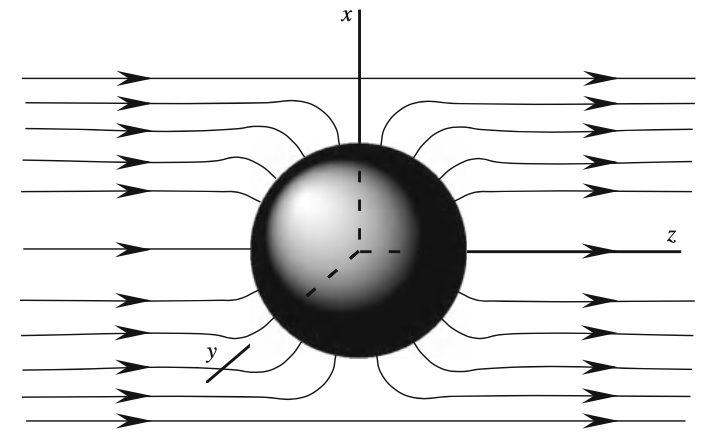
\includegraphics[scale=0.4]{Imagenes/Esfera_Compo_Electrico.png}
%     \caption{El campo eléctrico en la vecindad de una esfera colocada en un campo uniforme externo cambiará, pero el campo alejado de la esfera permanecerá casi uniforme.}
%     \label{fig:figura_esfera_aterrizada}
% \end{figure}

% \textbf{Queremos encontrar el potencial electrostático en todas partes fuera de la esfera}.
% \par
% Eligiendo que el campo esté en la dirección $z$ positiva y colocando el centro de la esfera en el origen, tendremos un problema que presenta simetría azimutal. Por lo tanto, la solución general viene dada por la ec. (\ref{eq:ecuacion_26_29}). Los límites por fuera de la esfera consisten en la esfera misma así como en el infinito. El campo eléctrico en el infinito es el campo uniforme original, porque el campo debido a las cargas inducidas en la esfera desaparece en el infinito. El potencial de este campo (en el infinito) se puede deducir de:
% \begin{align*}
% \vb{E} &= E_{0} \, \vu{e}_{z} = - \grad{\Phi} \\[0.5em]
% \Rightarrow \hspace{0.2cm} E_{0} &= - \pdv{\Phi}{z}, \hspace{1cm} \pdv{\Phi}{x} = \pdv{\Phi}{y} = 0
% \end{align*}
% Por lo tanto, el potencial en el infinito es independiente de $x$ e $y$, y se puede escribir como:
% \begin{align*}
% \Phi (r, \theta) &= - E_{0} \, z = \\[0.5em]
% &= - E_{0} \, r \, \cos \theta = \\[0.5em]
% &= - E_{0} \, r \, P_{1} (\cos \theta) \hspace{1cm} \mbox{para } r \to \infty
% \end{align*}
% Por lo tanto, el potencial en el infinito es independiente de $x$ e $y$, y se puede escribir como:


\end{document}